\section{Memory Scaling Behavior}

\subsection{Overview}

Scaling has been a key driver behind the continuous improvement of foundation models, where increasing model capacity, training data, and computation often leads to predictable gains in general capabilities~\cite{kaplan2020scalinglawsneurallanguage}.
However, for memory foundation models, it remains unclear whether native memory capabilities exhibit similar scaling behavior.
Exploring such scaling behavior is critical, as it reveals whether memory capability can continue to improve with scale and provides guidance for the design of larger memory foundation models.
In particular, memory-related training and the capacity of native memory states are two important factors that may influence memory capability, motivating us to explore scaling behavior along these two aspects.

In this work, we study memory scaling along both dimensions.
Data and training scaling explores how memory capability changes with continued exposure to memory-related post-training data, while memory capacity scaling studies the impact of increasing the capacity of native memory states.
They allow us to characterize how native memory capability evolves with additional training and expanded memory capacity.


\subsection{Scaling Protocol}

We conduct all scaling experiments based on MemT-1.0-Nano under a controlled experimental protocol.
We explore two scaling aspects, including data and training scaling and memory capacity scaling.
The backbone architecture, training objectives, and evaluation protocol are kept consistent across different configurations unless otherwise specified.
We evaluate memory capability using the same memory benchmarks to characterize performance changes across different scales.

Specifically, for data and training scaling, we evaluate checkpoints along a continuous post-training trajectory spanning two consecutive epochs over the same corpus.
The model architecture and training corpus remain fixed, while cumulative training exposure and optimization steps increase throughout training.
For memory capacity scaling, we vary the number of memory experts in MoS to expand native memory capacity, while keeping the remaining architectural components and training configurations consistent.
By examining the resulting performance curves, we investigate how native memory capability evolves with additional post-training and increased memory capacity.

\subsection{Data and Training Scaling}

We explore whether additional exposure to memory-related post-training data improves memory capability at a fixed model capacity.
Starting from the CPT checkpoint, we follow a single MemT-1.0-Nano training trajectory for two epochs over the same post-training corpus.
\begin{figure}[t]
    \centering
    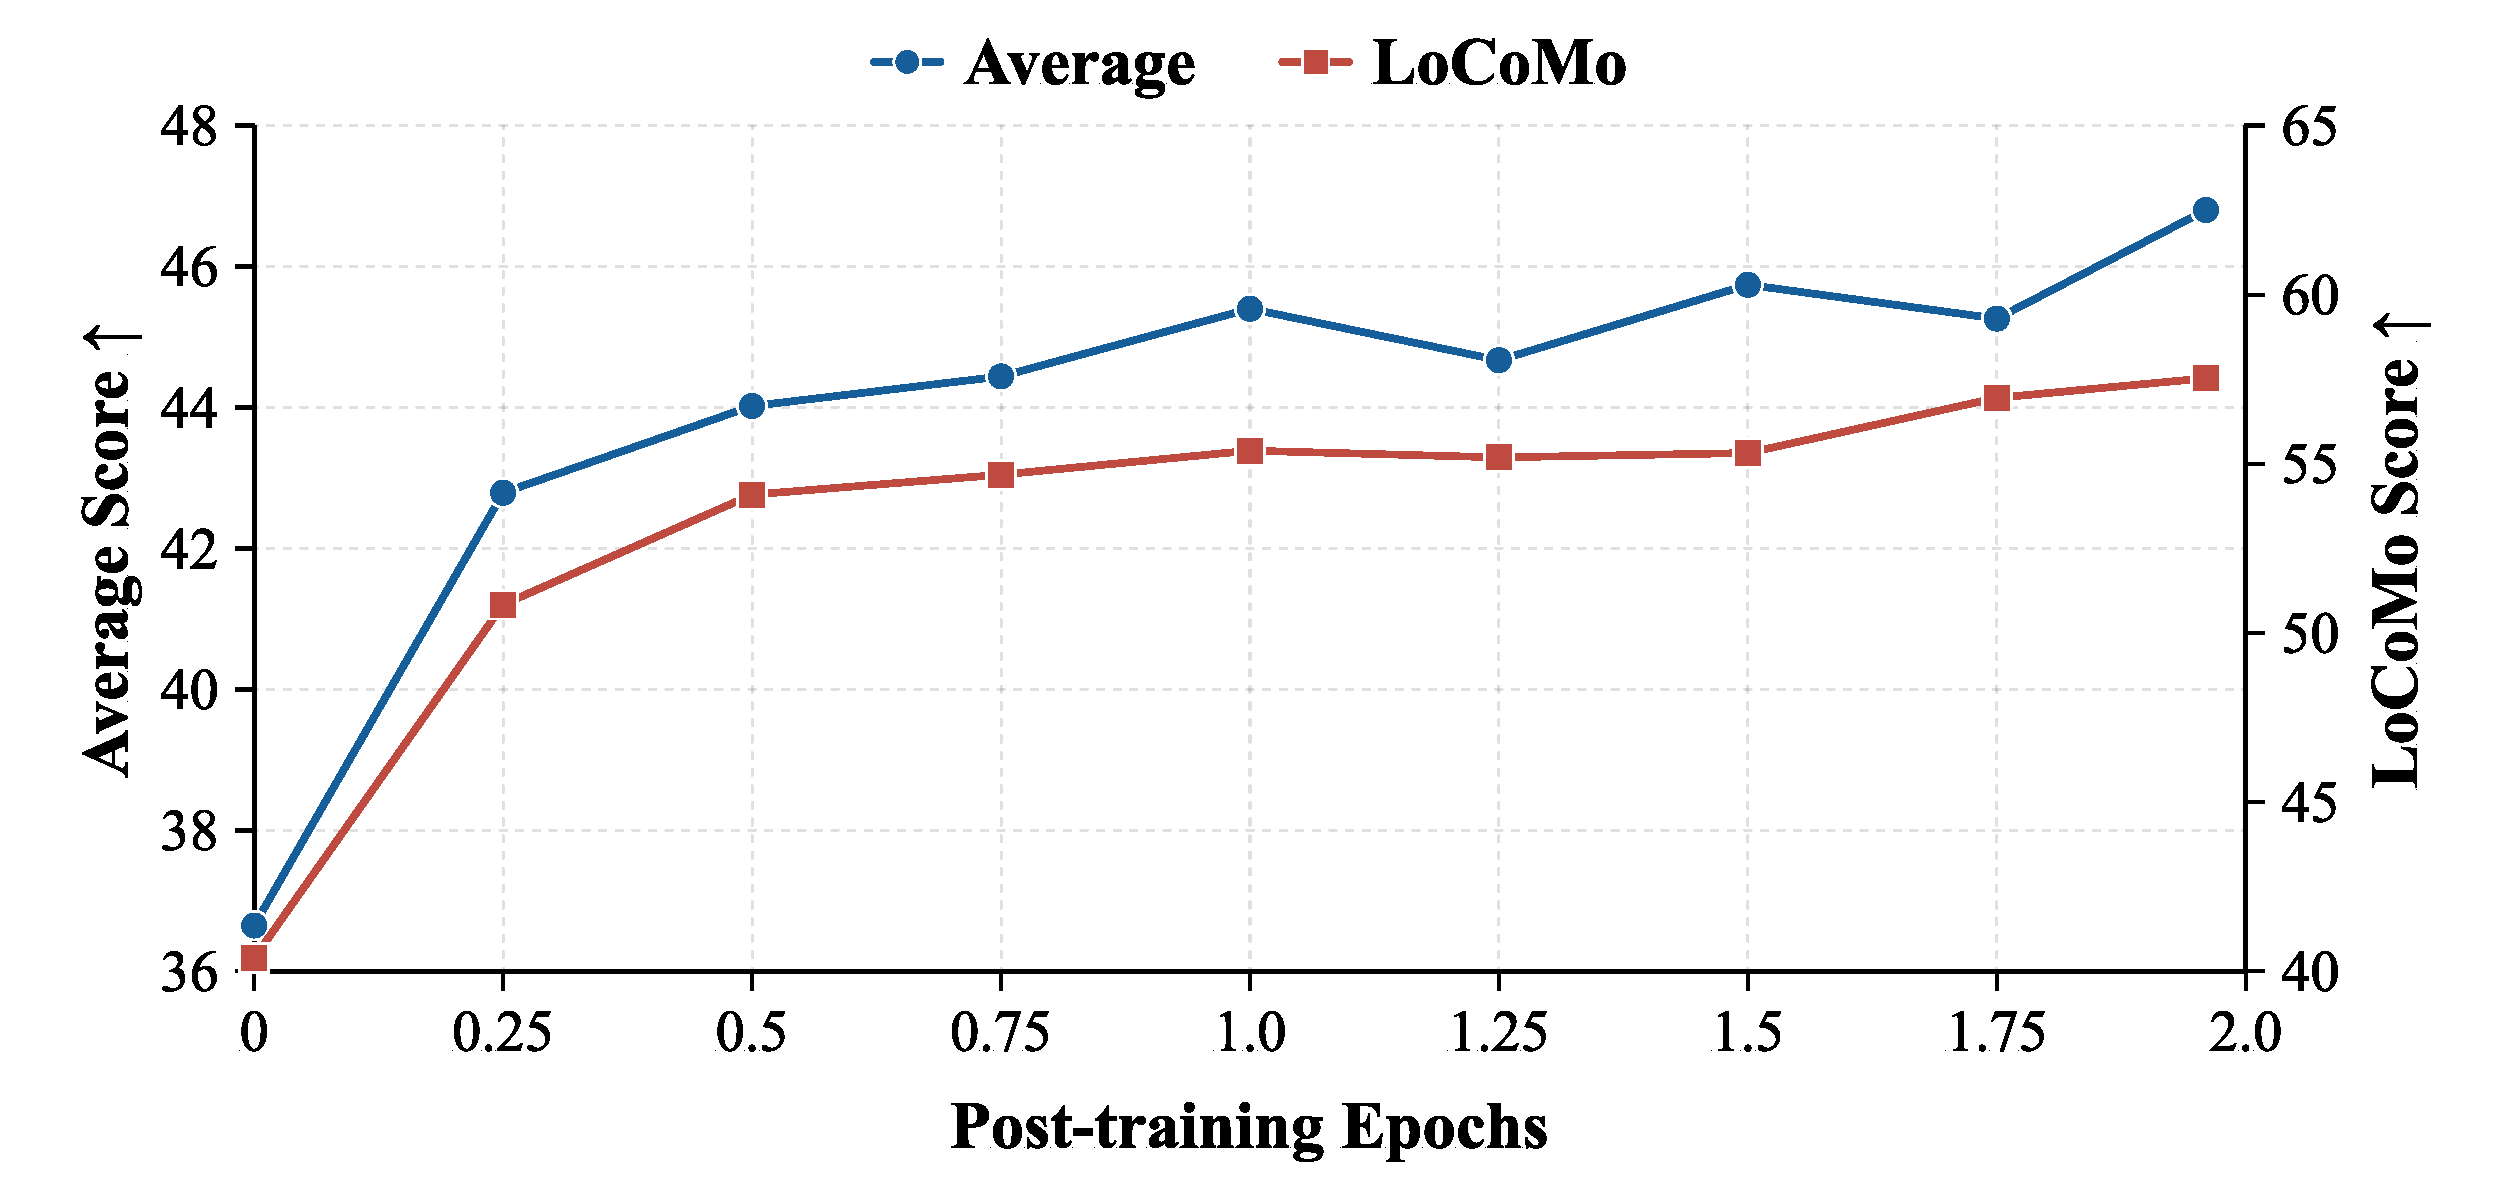
\includegraphics[width=0.8\linewidth]{figures/scaling_data.pdf}
    \vspace{-0.2cm}
    \caption{Data and training scaling of MemT-1.0-Nano.
    Memory performance over two consecutive post-training epochs.
    Blue circles show the average score on the left axis, and red squares show LoCoMo accuracy on the right axis.}
    \vspace{-0.4cm}
    \label{fig:training_data_scaling}
\end{figure}
Figure~\ref{fig:training_data_scaling} shows that memory performance generally improves with additional post-training.
Across the sampled checkpoints, the average score increases from 36.65 to 46.80, with intermediate fluctuations.
Most of this gain arrives early: the average score rises steeply within the first quarter epoch and continues to climb over the remainder of the first epoch, reaching 45.40 by its end, while LoCoMo improves from 40.39 to 55.39 over the same span.
This pattern is consistent with rapid adaptation of the CPT-initialized memory modules to downstream query answering, after which the increments shrink steadily but do not disappear.
In the second epoch, the final sampled checkpoint reaches 46.80 on average and 57.53 on LoCoMo, an improvement over the last sampled checkpoint of the first epoch despite intermediate fluctuations.
These gains indicate remaining room for optimization at fixed memory capacity, even when training revisits previously seen data.
In summary, continued exposure to memory-related post-training data can improve native memory capability, with further gains achievable across epochs without increasing model capacity.

\subsection{Memory Capacity Scaling}

Following 400 steps of CPT, we explore memory capacity scaling during post-training by comparing MoS configurations with 2 and 4 memory experts.
We evaluate both of them at 200, 3,400, and 5,500 post-training steps, reporting the average score alongside the LoCoMo score.
The results are presented in Figure~\ref{fig:memory_capacity_scaling}.
The 4-expert configuration consistently outperforms the 2-expert configuration across all three checkpoints, with relatively modest gains of 0.41 points in the average score and 1.42 points on LoCoMo at 200 post-training steps.
At 3,400 and 5,500 steps, increasing the number of experts improves the average score by 2.01 and 2.69 points, respectively, and LoCoMo by 3.25 and 2.20 points.
The 4-expert configuration continues to improve between these later checkpoints, with its average score increasing from 44.29 to 44.68 and its LoCoMo score rising from 53.51 to 55.58.
These results suggest that expanding memory capacity through additional experts benefits downstream performance, with larger gains at the later post-training checkpoints than at 200 steps.


\begin{figure}[t]
    \centering
    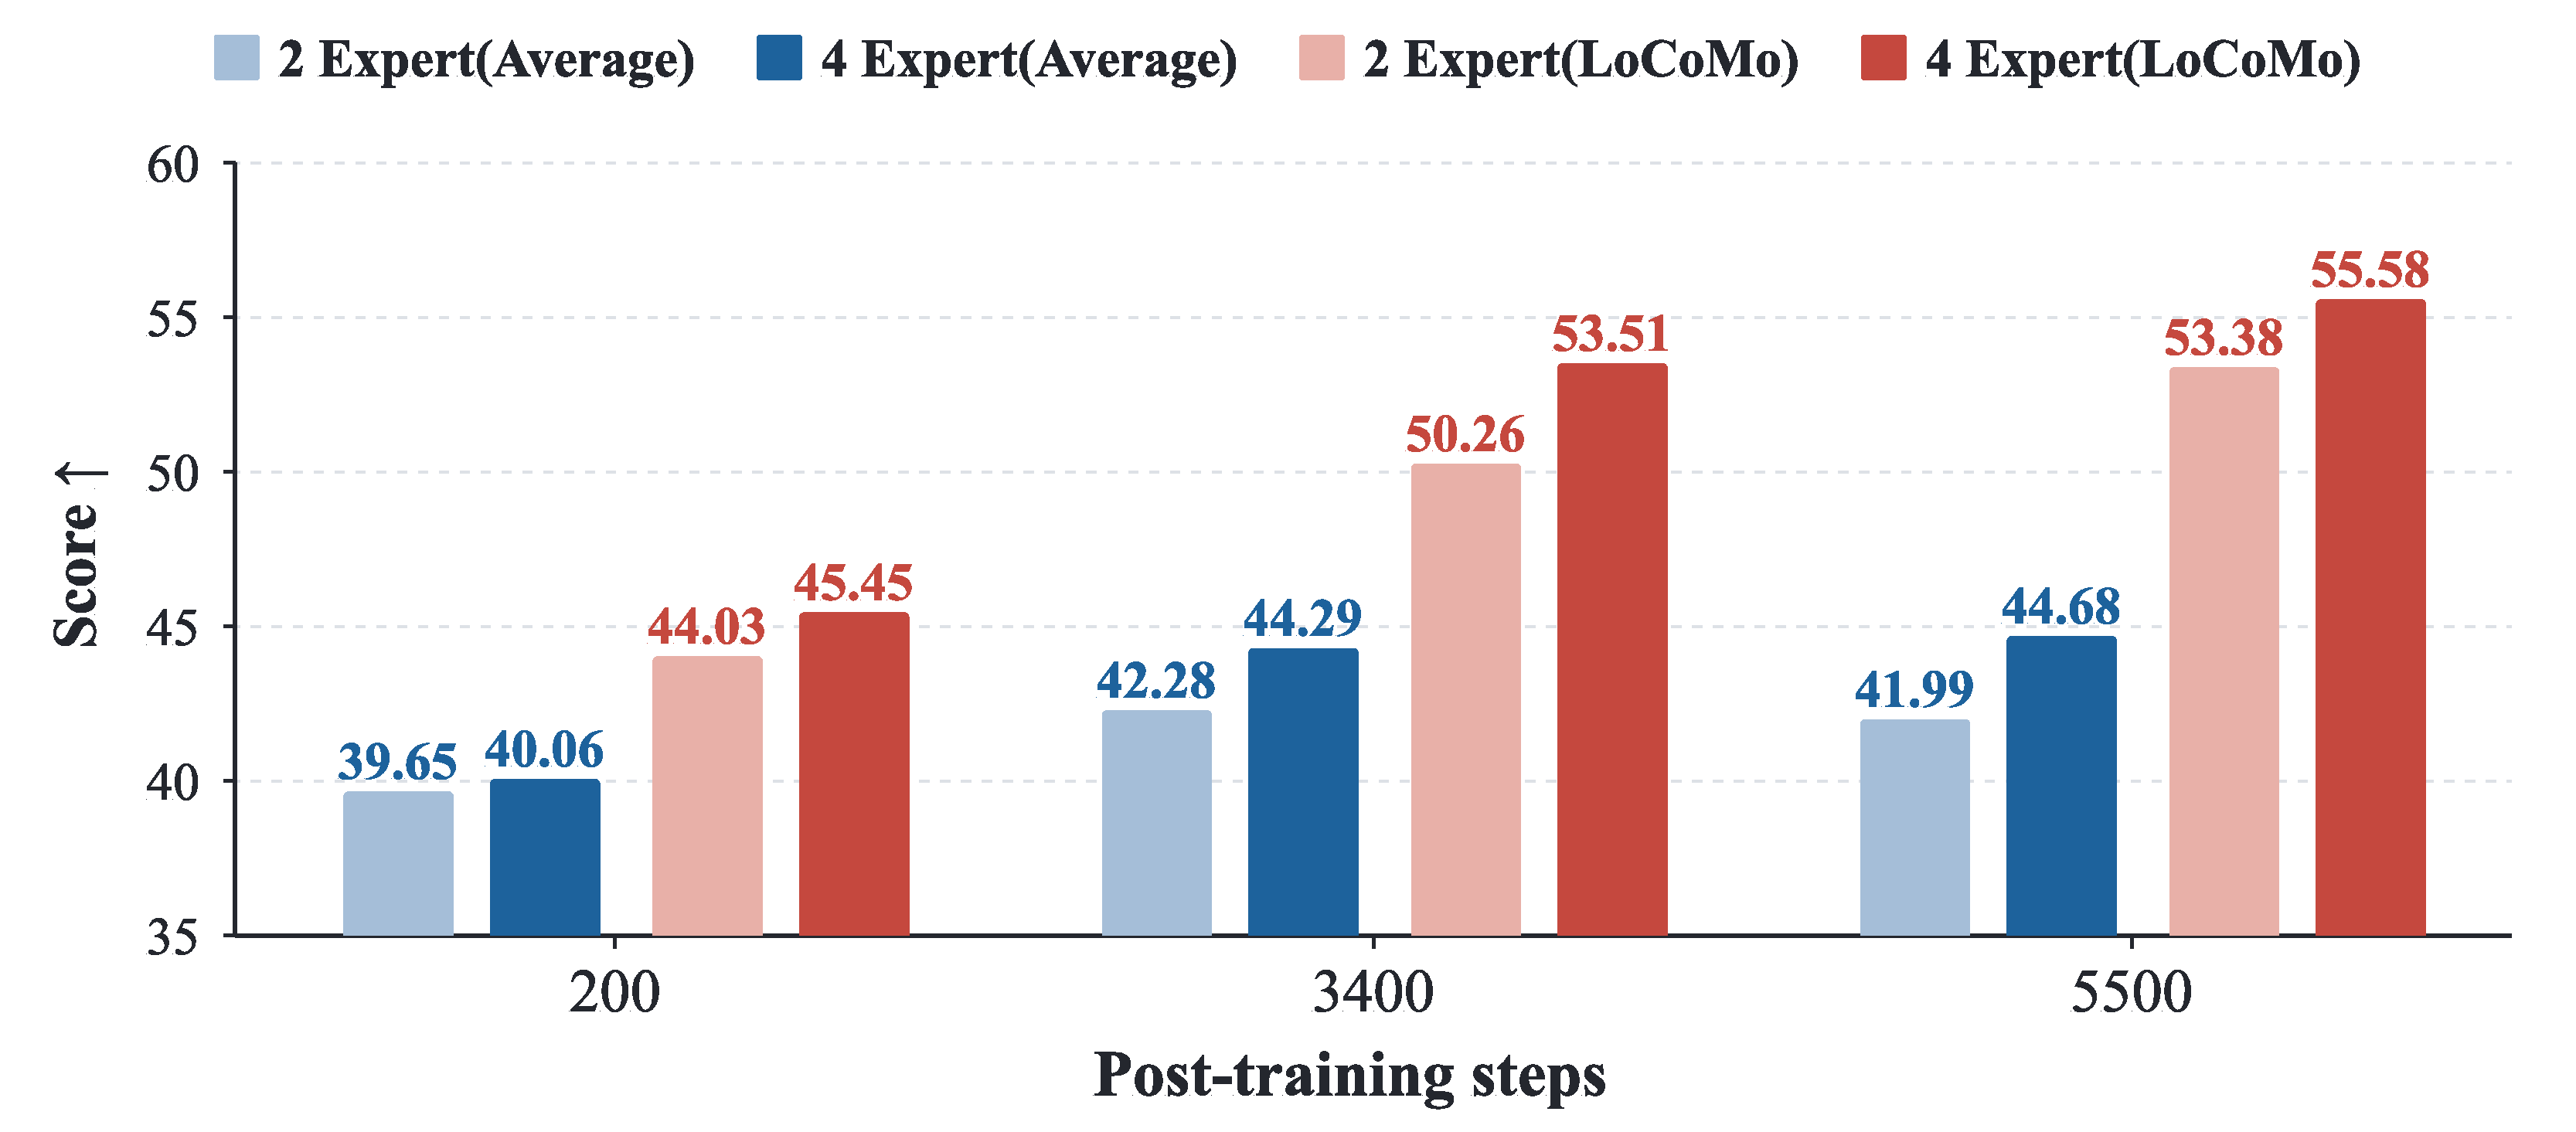
\includegraphics[width=0.88\linewidth]{figures/memory_capacity.pdf}
    \vspace{-0.2cm}
    \caption{Memory capacity scaling during post-training after 400 CPT steps. We compare MoS configurations with 2 and 4 memory experts at matched post-training steps, reporting the average score and the LoCoMo score.}
    \vspace{-0.4cm}
    \label{fig:memory_capacity_scaling}
\end{figure}